\documentclass{article} % For LaTeX2e
\usepackage{iclr2022_conference,times}
% Optional math commands from https://github.com/goodfeli/dlbook_notation.
%%%%% NEW MATH DEFINITIONS %%%%%

\usepackage{amsmath,amsfonts,bm}

% Mark sections of captions for referring to divisions of figures
\newcommand{\figleft}{{\em (Left)}}
\newcommand{\figcenter}{{\em (Center)}}
\newcommand{\figright}{{\em (Right)}}
\newcommand{\figtop}{{\em (Top)}}
\newcommand{\figbottom}{{\em (Bottom)}}
\newcommand{\captiona}{{\em (a)}}
\newcommand{\captionb}{{\em (b)}}
\newcommand{\captionc}{{\em (c)}}
\newcommand{\captiond}{{\em (d)}}

% Highlight a newly defined term
\newcommand{\newterm}[1]{{\bf #1}}


% Figure reference, lower-case.
\def\figref#1{figure~\ref{#1}}
% Figure reference, capital. For start of sentence
\def\Figref#1{Figure~\ref{#1}}
\def\twofigref#1#2{figures \ref{#1} and \ref{#2}}
\def\quadfigref#1#2#3#4{figures \ref{#1}, \ref{#2}, \ref{#3} and \ref{#4}}
% Section reference, lower-case.
\def\secref#1{section~\ref{#1}}
% Section reference, capital.
\def\Secref#1{Section~\ref{#1}}
% Reference to two sections.
\def\twosecrefs#1#2{sections \ref{#1} and \ref{#2}}
% Reference to three sections.
\def\secrefs#1#2#3{sections \ref{#1}, \ref{#2} and \ref{#3}}
% Reference to an equation, lower-case.
\def\eqref#1{equation~\ref{#1}}
% Reference to an equation, upper case
\def\Eqref#1{Equation~\ref{#1}}
% A raw reference to an equation---avoid using if possible
\def\plaineqref#1{\ref{#1}}
% Reference to a chapter, lower-case.
\def\chapref#1{chapter~\ref{#1}}
% Reference to an equation, upper case.
\def\Chapref#1{Chapter~\ref{#1}}
% Reference to a range of chapters
\def\rangechapref#1#2{chapters\ref{#1}--\ref{#2}}
% Reference to an algorithm, lower-case.
\def\algref#1{algorithm~\ref{#1}}
% Reference to an algorithm, upper case.
\def\Algref#1{Algorithm~\ref{#1}}
\def\twoalgref#1#2{algorithms \ref{#1} and \ref{#2}}
\def\Twoalgref#1#2{Algorithms \ref{#1} and \ref{#2}}
% Reference to a part, lower case
\def\partref#1{part~\ref{#1}}
% Reference to a part, upper case
\def\Partref#1{Part~\ref{#1}}
\def\twopartref#1#2{parts \ref{#1} and \ref{#2}}

\def\ceil#1{\lceil #1 \rceil}
\def\floor#1{\lfloor #1 \rfloor}
\def\1{\bm{1}}
\newcommand{\train}{\mathcal{D}}
\newcommand{\valid}{\mathcal{D_{\mathrm{valid}}}}
\newcommand{\test}{\mathcal{D_{\mathrm{test}}}}

\def\eps{{\epsilon}}


% Random variables
\def\reta{{\textnormal{$\eta$}}}
\def\ra{{\textnormal{a}}}
\def\rb{{\textnormal{b}}}
\def\rc{{\textnormal{c}}}
\def\rd{{\textnormal{d}}}
\def\re{{\textnormal{e}}}
\def\rf{{\textnormal{f}}}
\def\rg{{\textnormal{g}}}
\def\rh{{\textnormal{h}}}
\def\ri{{\textnormal{i}}}
\def\rj{{\textnormal{j}}}
\def\rk{{\textnormal{k}}}
\def\rl{{\textnormal{l}}}
% rm is already a command, just don't name any random variables m
\def\rn{{\textnormal{n}}}
\def\ro{{\textnormal{o}}}
\def\rp{{\textnormal{p}}}
\def\rq{{\textnormal{q}}}
\def\rr{{\textnormal{r}}}
\def\rs{{\textnormal{s}}}
\def\rt{{\textnormal{t}}}
\def\ru{{\textnormal{u}}}
\def\rv{{\textnormal{v}}}
\def\rw{{\textnormal{w}}}
\def\rx{{\textnormal{x}}}
\def\ry{{\textnormal{y}}}
\def\rz{{\textnormal{z}}}

% Random vectors
\def\rvepsilon{{\mathbf{\epsilon}}}
\def\rvtheta{{\mathbf{\theta}}}
\def\rva{{\mathbf{a}}}
\def\rvb{{\mathbf{b}}}
\def\rvc{{\mathbf{c}}}
\def\rvd{{\mathbf{d}}}
\def\rve{{\mathbf{e}}}
\def\rvf{{\mathbf{f}}}
\def\rvg{{\mathbf{g}}}
\def\rvh{{\mathbf{h}}}
\def\rvu{{\mathbf{i}}}
\def\rvj{{\mathbf{j}}}
\def\rvk{{\mathbf{k}}}
\def\rvl{{\mathbf{l}}}
\def\rvm{{\mathbf{m}}}
\def\rvn{{\mathbf{n}}}
\def\rvo{{\mathbf{o}}}
\def\rvp{{\mathbf{p}}}
\def\rvq{{\mathbf{q}}}
\def\rvr{{\mathbf{r}}}
\def\rvs{{\mathbf{s}}}
\def\rvt{{\mathbf{t}}}
\def\rvu{{\mathbf{u}}}
\def\rvv{{\mathbf{v}}}
\def\rvw{{\mathbf{w}}}
\def\rvx{{\mathbf{x}}}
\def\rvy{{\mathbf{y}}}
\def\rvz{{\mathbf{z}}}

% Elements of random vectors
\def\erva{{\textnormal{a}}}
\def\ervb{{\textnormal{b}}}
\def\ervc{{\textnormal{c}}}
\def\ervd{{\textnormal{d}}}
\def\erve{{\textnormal{e}}}
\def\ervf{{\textnormal{f}}}
\def\ervg{{\textnormal{g}}}
\def\ervh{{\textnormal{h}}}
\def\ervi{{\textnormal{i}}}
\def\ervj{{\textnormal{j}}}
\def\ervk{{\textnormal{k}}}
\def\ervl{{\textnormal{l}}}
\def\ervm{{\textnormal{m}}}
\def\ervn{{\textnormal{n}}}
\def\ervo{{\textnormal{o}}}
\def\ervp{{\textnormal{p}}}
\def\ervq{{\textnormal{q}}}
\def\ervr{{\textnormal{r}}}
\def\ervs{{\textnormal{s}}}
\def\ervt{{\textnormal{t}}}
\def\ervu{{\textnormal{u}}}
\def\ervv{{\textnormal{v}}}
\def\ervw{{\textnormal{w}}}
\def\ervx{{\textnormal{x}}}
\def\ervy{{\textnormal{y}}}
\def\ervz{{\textnormal{z}}}

% Random matrices
\def\rmA{{\mathbf{A}}}
\def\rmB{{\mathbf{B}}}
\def\rmC{{\mathbf{C}}}
\def\rmD{{\mathbf{D}}}
\def\rmE{{\mathbf{E}}}
\def\rmF{{\mathbf{F}}}
\def\rmG{{\mathbf{G}}}
\def\rmH{{\mathbf{H}}}
\def\rmI{{\mathbf{I}}}
\def\rmJ{{\mathbf{J}}}
\def\rmK{{\mathbf{K}}}
\def\rmL{{\mathbf{L}}}
\def\rmM{{\mathbf{M}}}
\def\rmN{{\mathbf{N}}}
\def\rmO{{\mathbf{O}}}
\def\rmP{{\mathbf{P}}}
\def\rmQ{{\mathbf{Q}}}
\def\rmR{{\mathbf{R}}}
\def\rmS{{\mathbf{S}}}
\def\rmT{{\mathbf{T}}}
\def\rmU{{\mathbf{U}}}
\def\rmV{{\mathbf{V}}}
\def\rmW{{\mathbf{W}}}
\def\rmX{{\mathbf{X}}}
\def\rmY{{\mathbf{Y}}}
\def\rmZ{{\mathbf{Z}}}

% Elements of random matrices
\def\ermA{{\textnormal{A}}}
\def\ermB{{\textnormal{B}}}
\def\ermC{{\textnormal{C}}}
\def\ermD{{\textnormal{D}}}
\def\ermE{{\textnormal{E}}}
\def\ermF{{\textnormal{F}}}
\def\ermG{{\textnormal{G}}}
\def\ermH{{\textnormal{H}}}
\def\ermI{{\textnormal{I}}}
\def\ermJ{{\textnormal{J}}}
\def\ermK{{\textnormal{K}}}
\def\ermL{{\textnormal{L}}}
\def\ermM{{\textnormal{M}}}
\def\ermN{{\textnormal{N}}}
\def\ermO{{\textnormal{O}}}
\def\ermP{{\textnormal{P}}}
\def\ermQ{{\textnormal{Q}}}
\def\ermR{{\textnormal{R}}}
\def\ermS{{\textnormal{S}}}
\def\ermT{{\textnormal{T}}}
\def\ermU{{\textnormal{U}}}
\def\ermV{{\textnormal{V}}}
\def\ermW{{\textnormal{W}}}
\def\ermX{{\textnormal{X}}}
\def\ermY{{\textnormal{Y}}}
\def\ermZ{{\textnormal{Z}}}

% Vectors
\def\vzero{{\bm{0}}}
\def\vone{{\bm{1}}}
\def\vmu{{\bm{\mu}}}
\def\vtheta{{\bm{\theta}}}
\def\va{{\bm{a}}}
\def\vb{{\bm{b}}}
\def\vc{{\bm{c}}}
\def\vd{{\bm{d}}}
\def\ve{{\bm{e}}}
\def\vf{{\bm{f}}}
\def\vg{{\bm{g}}}
\def\vh{{\bm{h}}}
\def\vi{{\bm{i}}}
\def\vj{{\bm{j}}}
\def\vk{{\bm{k}}}
\def\vl{{\bm{l}}}
\def\vm{{\bm{m}}}
\def\vn{{\bm{n}}}
\def\vo{{\bm{o}}}
\def\vp{{\bm{p}}}
\def\vq{{\bm{q}}}
\def\vr{{\bm{r}}}
\def\vs{{\bm{s}}}
\def\vt{{\bm{t}}}
\def\vu{{\bm{u}}}
\def\vv{{\bm{v}}}
\def\vw{{\bm{w}}}
\def\vx{{\bm{x}}}
\def\vy{{\bm{y}}}
\def\vz{{\bm{z}}}

% Elements of vectors
\def\evalpha{{\alpha}}
\def\evbeta{{\beta}}
\def\evepsilon{{\epsilon}}
\def\evlambda{{\lambda}}
\def\evomega{{\omega}}
\def\evmu{{\mu}}
\def\evpsi{{\psi}}
\def\evsigma{{\sigma}}
\def\evtheta{{\theta}}
\def\eva{{a}}
\def\evb{{b}}
\def\evc{{c}}
\def\evd{{d}}
\def\eve{{e}}
\def\evf{{f}}
\def\evg{{g}}
\def\evh{{h}}
\def\evi{{i}}
\def\evj{{j}}
\def\evk{{k}}
\def\evl{{l}}
\def\evm{{m}}
\def\evn{{n}}
\def\evo{{o}}
\def\evp{{p}}
\def\evq{{q}}
\def\evr{{r}}
\def\evs{{s}}
\def\evt{{t}}
\def\evu{{u}}
\def\evv{{v}}
\def\evw{{w}}
\def\evx{{x}}
\def\evy{{y}}
\def\evz{{z}}

% Matrix
\def\mA{{\bm{A}}}
\def\mB{{\bm{B}}}
\def\mC{{\bm{C}}}
\def\mD{{\bm{D}}}
\def\mE{{\bm{E}}}
\def\mF{{\bm{F}}}
\def\mG{{\bm{G}}}
\def\mH{{\bm{H}}}
\def\mI{{\bm{I}}}
\def\mJ{{\bm{J}}}
\def\mK{{\bm{K}}}
\def\mL{{\bm{L}}}
\def\mM{{\bm{M}}}
\def\mN{{\bm{N}}}
\def\mO{{\bm{O}}}
\def\mP{{\bm{P}}}
\def\mQ{{\bm{Q}}}
\def\mR{{\bm{R}}}
\def\mS{{\bm{S}}}
\def\mT{{\bm{T}}}
\def\mU{{\bm{U}}}
\def\mV{{\bm{V}}}
\def\mW{{\bm{W}}}
\def\mX{{\bm{X}}}
\def\mY{{\bm{Y}}}
\def\mZ{{\bm{Z}}}
\def\mBeta{{\bm{\beta}}}
\def\mPhi{{\bm{\Phi}}}
\def\mLambda{{\bm{\Lambda}}}
\def\mSigma{{\bm{\Sigma}}}

% Tensor
\DeclareMathAlphabet{\mathsfit}{\encodingdefault}{\sfdefault}{m}{sl}
\SetMathAlphabet{\mathsfit}{bold}{\encodingdefault}{\sfdefault}{bx}{n}
\newcommand{\tens}[1]{\bm{\mathsfit{#1}}}
\def\tA{{\tens{A}}}
\def\tB{{\tens{B}}}
\def\tC{{\tens{C}}}
\def\tD{{\tens{D}}}
\def\tE{{\tens{E}}}
\def\tF{{\tens{F}}}
\def\tG{{\tens{G}}}
\def\tH{{\tens{H}}}
\def\tI{{\tens{I}}}
\def\tJ{{\tens{J}}}
\def\tK{{\tens{K}}}
\def\tL{{\tens{L}}}
\def\tM{{\tens{M}}}
\def\tN{{\tens{N}}}
\def\tO{{\tens{O}}}
\def\tP{{\tens{P}}}
\def\tQ{{\tens{Q}}}
\def\tR{{\tens{R}}}
\def\tS{{\tens{S}}}
\def\tT{{\tens{T}}}
\def\tU{{\tens{U}}}
\def\tV{{\tens{V}}}
\def\tW{{\tens{W}}}
\def\tX{{\tens{X}}}
\def\tY{{\tens{Y}}}
\def\tZ{{\tens{Z}}}


% Graph
\def\gA{{\mathcal{A}}}
\def\gB{{\mathcal{B}}}
\def\gC{{\mathcal{C}}}
\def\gD{{\mathcal{D}}}
\def\gE{{\mathcal{E}}}
\def\gF{{\mathcal{F}}}
\def\gG{{\mathcal{G}}}
\def\gH{{\mathcal{H}}}
\def\gI{{\mathcal{I}}}
\def\gJ{{\mathcal{J}}}
\def\gK{{\mathcal{K}}}
\def\gL{{\mathcal{L}}}
\def\gM{{\mathcal{M}}}
\def\gN{{\mathcal{N}}}
\def\gO{{\mathcal{O}}}
\def\gP{{\mathcal{P}}}
\def\gQ{{\mathcal{Q}}}
\def\gR{{\mathcal{R}}}
\def\gS{{\mathcal{S}}}
\def\gT{{\mathcal{T}}}
\def\gU{{\mathcal{U}}}
\def\gV{{\mathcal{V}}}
\def\gW{{\mathcal{W}}}
\def\gX{{\mathcal{X}}}
\def\gY{{\mathcal{Y}}}
\def\gZ{{\mathcal{Z}}}

% Sets
\def\sA{{\mathbb{A}}}
\def\sB{{\mathbb{B}}}
\def\sC{{\mathbb{C}}}
\def\sD{{\mathbb{D}}}
% Don't use a set called E, because this would be the same as our symbol
% for expectation.
\def\sF{{\mathbb{F}}}
\def\sG{{\mathbb{G}}}
\def\sH{{\mathbb{H}}}
\def\sI{{\mathbb{I}}}
\def\sJ{{\mathbb{J}}}
\def\sK{{\mathbb{K}}}
\def\sL{{\mathbb{L}}}
\def\sM{{\mathbb{M}}}
\def\sN{{\mathbb{N}}}
\def\sO{{\mathbb{O}}}
\def\sP{{\mathbb{P}}}
\def\sQ{{\mathbb{Q}}}
\def\sR{{\mathbb{R}}}
\def\sS{{\mathbb{S}}}
\def\sT{{\mathbb{T}}}
\def\sU{{\mathbb{U}}}
\def\sV{{\mathbb{V}}}
\def\sW{{\mathbb{W}}}
\def\sX{{\mathbb{X}}}
\def\sY{{\mathbb{Y}}}
\def\sZ{{\mathbb{Z}}}

% Entries of a matrix
\def\emLambda{{\Lambda}}
\def\emA{{A}}
\def\emB{{B}}
\def\emC{{C}}
\def\emD{{D}}
\def\emE{{E}}
\def\emF{{F}}
\def\emG{{G}}
\def\emH{{H}}
\def\emI{{I}}
\def\emJ{{J}}
\def\emK{{K}}
\def\emL{{L}}
\def\emM{{M}}
\def\emN{{N}}
\def\emO{{O}}
\def\emP{{P}}
\def\emQ{{Q}}
\def\emR{{R}}
\def\emS{{S}}
\def\emT{{T}}
\def\emU{{U}}
\def\emV{{V}}
\def\emW{{W}}
\def\emX{{X}}
\def\emY{{Y}}
\def\emZ{{Z}}
\def\emSigma{{\Sigma}}

% entries of a tensor
% Same font as tensor, without \bm wrapper
\newcommand{\etens}[1]{\mathsfit{#1}}
\def\etLambda{{\etens{\Lambda}}}
\def\etA{{\etens{A}}}
\def\etB{{\etens{B}}}
\def\etC{{\etens{C}}}
\def\etD{{\etens{D}}}
\def\etE{{\etens{E}}}
\def\etF{{\etens{F}}}
\def\etG{{\etens{G}}}
\def\etH{{\etens{H}}}
\def\etI{{\etens{I}}}
\def\etJ{{\etens{J}}}
\def\etK{{\etens{K}}}
\def\etL{{\etens{L}}}
\def\etM{{\etens{M}}}
\def\etN{{\etens{N}}}
\def\etO{{\etens{O}}}
\def\etP{{\etens{P}}}
\def\etQ{{\etens{Q}}}
\def\etR{{\etens{R}}}
\def\etS{{\etens{S}}}
\def\etT{{\etens{T}}}
\def\etU{{\etens{U}}}
\def\etV{{\etens{V}}}
\def\etW{{\etens{W}}}
\def\etX{{\etens{X}}}
\def\etY{{\etens{Y}}}
\def\etZ{{\etens{Z}}}

% The true underlying data generating distribution
\newcommand{\pdata}{p_{\rm{data}}}
% The empirical distribution defined by the training set
\newcommand{\ptrain}{\hat{p}_{\rm{data}}}
\newcommand{\Ptrain}{\hat{P}_{\rm{data}}}
% The model distribution
\newcommand{\pmodel}{p_{\rm{model}}}
\newcommand{\Pmodel}{P_{\rm{model}}}
\newcommand{\ptildemodel}{\tilde{p}_{\rm{model}}}
% Stochastic autoencoder distributions
\newcommand{\pencode}{p_{\rm{encoder}}}
\newcommand{\pdecode}{p_{\rm{decoder}}}
\newcommand{\precons}{p_{\rm{reconstruct}}}

\newcommand{\laplace}{\mathrm{Laplace}} % Laplace distribution

\newcommand{\E}{\mathbb{E}}
\newcommand{\Ls}{\mathcal{L}}
\newcommand{\R}{\mathbb{R}}
\newcommand{\emp}{\tilde{p}}
\newcommand{\lr}{\alpha}
\newcommand{\reg}{\lambda}
\newcommand{\rect}{\mathrm{rectifier}}
\newcommand{\softmax}{\mathrm{softmax}}
\newcommand{\sigmoid}{\sigma}
\newcommand{\softplus}{\zeta}
\newcommand{\KL}{D_{\mathrm{KL}}}
\newcommand{\Var}{\mathrm{Var}}
\newcommand{\standarderror}{\mathrm{SE}}
\newcommand{\Cov}{\mathrm{Cov}}
% Wolfram Mathworld says $L^2$ is for function spaces and $\ell^2$ is for vectors
% But then they seem to use $L^2$ for vectors throughout the site, and so does
% wikipedia.
\newcommand{\normlzero}{L^0}
\newcommand{\normlone}{L^1}
\newcommand{\normltwo}{L^2}
\newcommand{\normlp}{L^p}
\newcommand{\normmax}{L^\infty}

\newcommand{\parents}{Pa} % See usage in notation.tex. Chosen to match Daphne's book.

\DeclareMathOperator*{\argmax}{arg\,max}
\DeclareMathOperator*{\argmin}{arg\,min}

\DeclareMathOperator{\sign}{sign}
\DeclareMathOperator{\Tr}{Tr}
\let\ab\allowbreak


%######## APS360: Uncomment your submission name
\newcommand{\apsname}{Project Proposal}
%\newcommand{\apsname}{Progress Report}
%\newcommand{\apsname}{Final Report}

%######## APS360: Put your Group Number here
\newcommand{\gpnumber}{6}

\usepackage{hyperref}
\usepackage{url}
\usepackage{graphicx}

%######## APS360: Put your project Title here
\title{APS360 Project Proposal}


%######## APS360: Put your names, student IDs and Emails here
\author{Junwon Kang  \\
Student\# 1007390958\\
\texttt{junwon.kang@mail.utoronto.ca} \\
\And
Mukund Hari \\
Student\# 1006999517 \\
\texttt{mukund.hari@mail.utoronto.ca} \\
\AND
John Angelou  \\
Student\# 1006722520 \\
\texttt{john.angelou@mail.utoronto.ca} \\
\And
Haoning Yuan \\
Student\# 1006702720 \\
\texttt{haoning.yuan@mail.utoronto.ca} \\
\AND
}

% The \author macro works with any number of authors. There are two commands
% used to separate the names and addresses of multiple authors: \And and \AND.
%
% Using \And between authors leaves it to \LaTeX{} to determine where to break
% the lines. Using \AND forces a linebreak at that point. So, if \LaTeX{}
% puts 3 of 4 authors names on the first line, and the last on the second
% line, try using \AND instead of \And before the third author name.

\newcommand{\fix}{\marginpar{FIX}}
\newcommand{\new}{\marginpar{NEW}}

\iclrfinalcopy 
%######## APS360: Document starts here
\begin{document}

\maketitle

\begin{abstract}
For this project, we aim to classify the first two generations of pokemon images using deep learning as a tool. Data used to train and test the model is obtained in two ways. Images of the first generation pokemon were obtained from the “7000 Labeled Pokemon” dataset from Kaggle.  Images for second generation pokemon were obtained by all group members through manual selection from the internet. The architecture the group proposes for the model will be a combination of alexNet, Visual Geometry Group 19, and ResNet-34 architecture. The baseline model used to compare our final model is a Support Vector Machine (SVM) classification model due to its relatively high accuracy within certain image sets. The group looks into some ethical considerations such as ethical issues in data collection and in using the model in detrimental ways. Some risks are also considered for this project such as splitting up the dataset in an unbalanced way, duplicate images, and members dropping APS360 course. 
%######## APS360: Do not change the next line. This shows your Main body page count.
----Total Pages: \pageref{last_page}
\end{abstract}

\section{Introduction}

Pokemon originated as a video game series in Japan in 1996, later coming to the Untied States in 1998 \citep{Britannica}. Since its original release, pokemon is now one of the most popular media franchises of all time and is the 3rd best selling video game franchise with over 440 million copies sold worldwide \citep{PokemonCompany}. In the games, there are fictional creatures called "pokemon" that come in many shapes and sizes. There are exactly 1008 pokemon in total spread between 9 different generations \citep{PokemonNum}. For this project, we scope down and focus on the first two generations of pokemon which is 251 pokemon in total. The goal of this project is to correctly classify images of pokemon within the first two generations using machine learning as a tool, specifically deep learning. Deep learning is a great approach for this project as this is mainly an image classification project. Pokemons have many different distinct features that put them apart, meaning there are many features to extract and use. Finally, using deep learning to classify images of pokemon has interesting implications for the future as it may advance pokemon games to the point where the player can get information about each pokemon by using mods to identify the pokemon in real time.

\section{Illustration}

Figure 1 contains an illustration of the overall idea and architecture of the model. 

\begin{figure}[h]
\begin{center}
\graphicspath{ {./imgs/} }
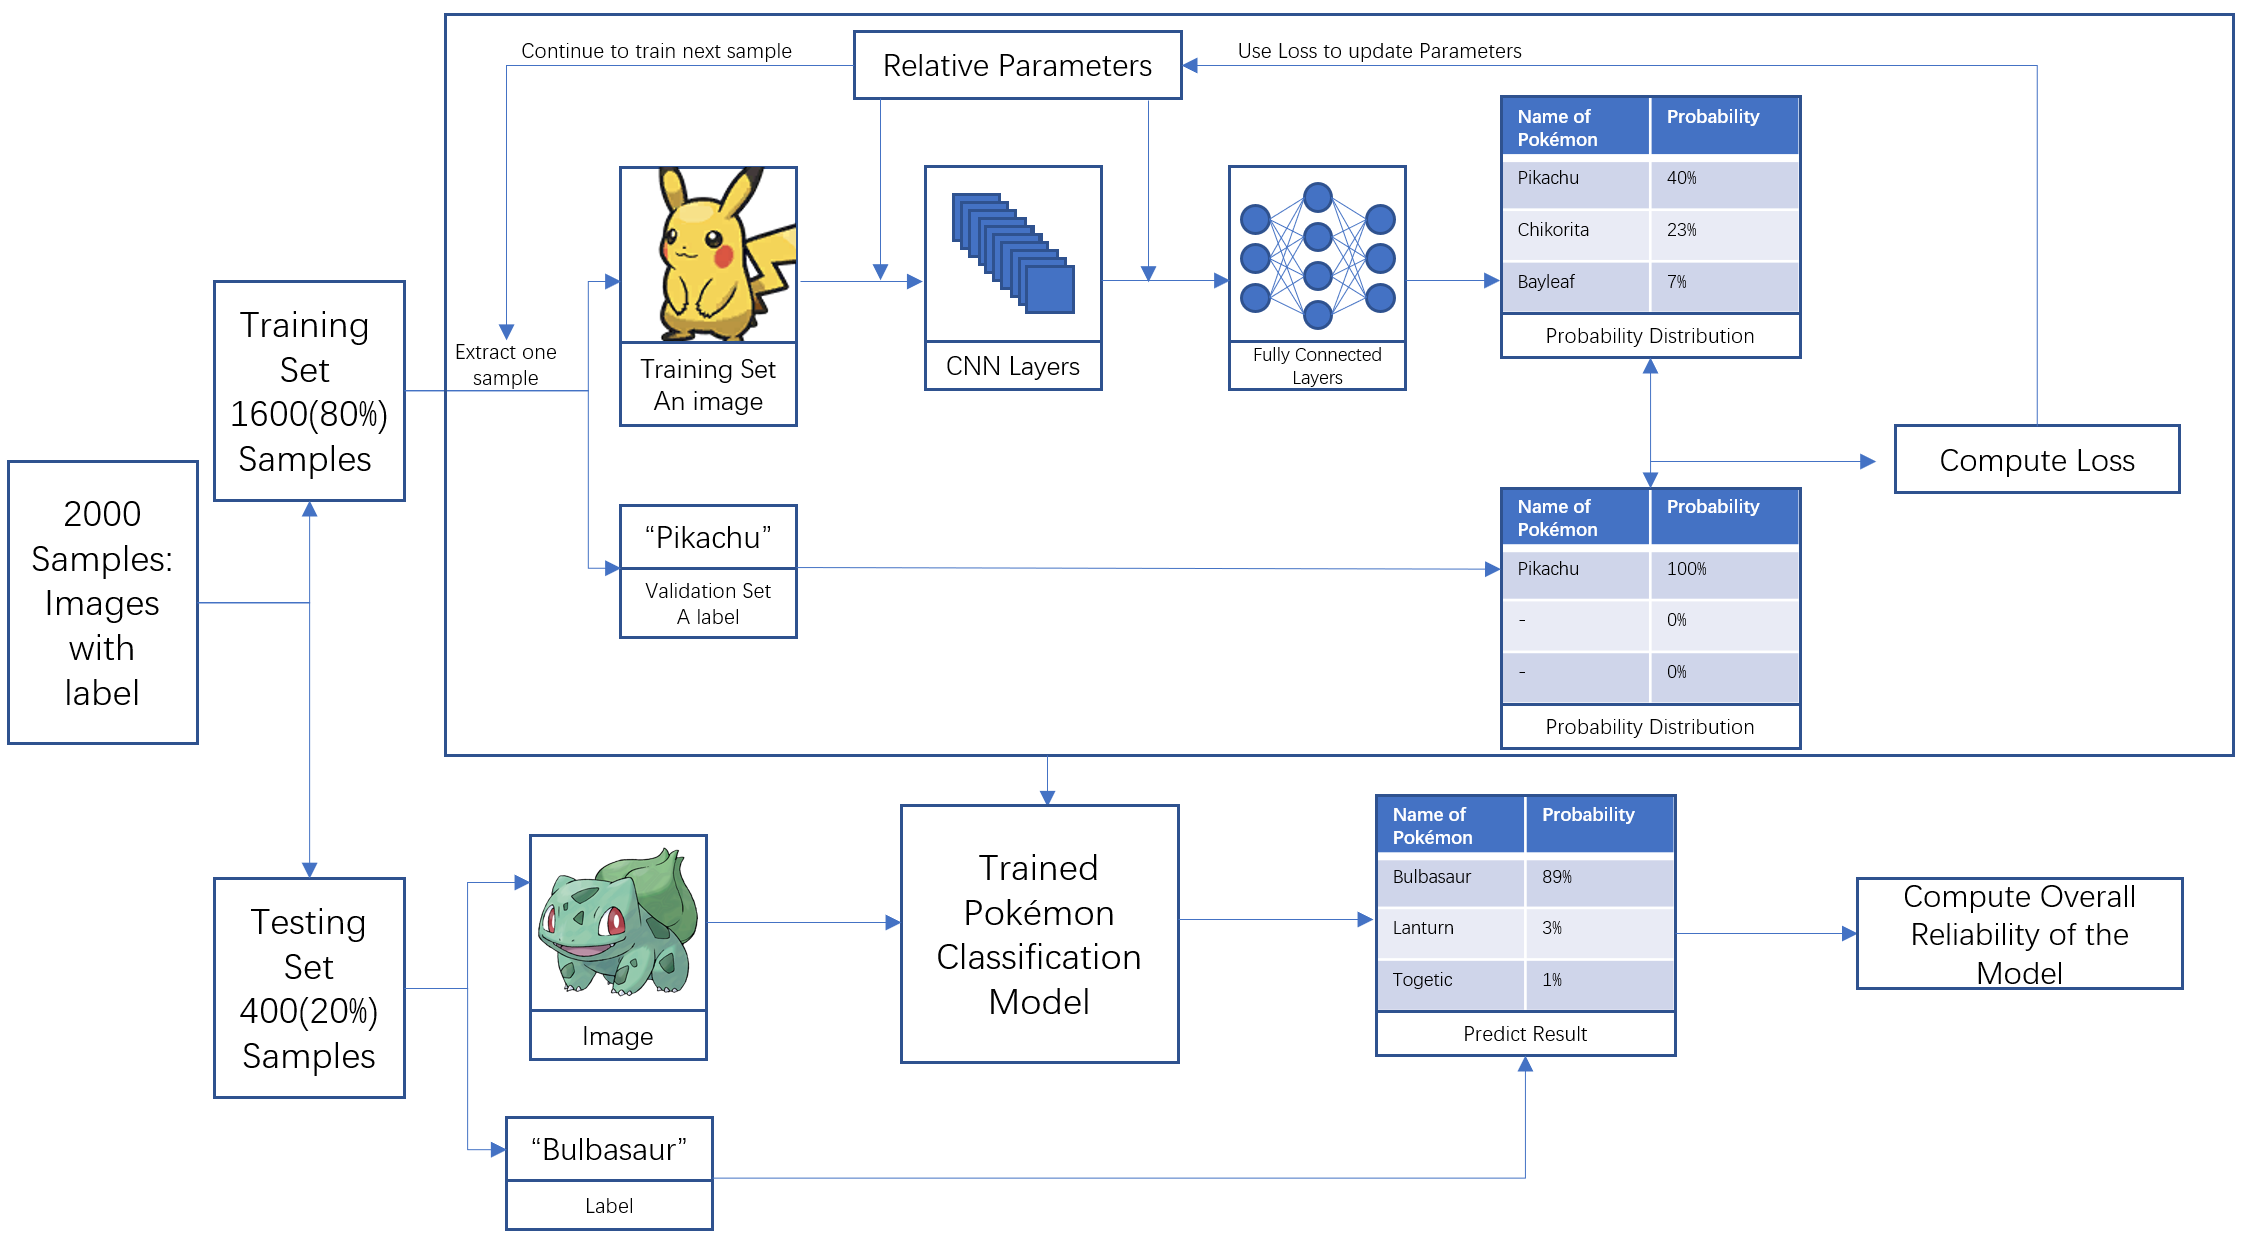
\includegraphics[width=\textwidth]{imgs/Modelillustration.png}
\end{center}
\caption{Overall idea and architecture of the model}
\end{figure}

\section{Background and Related Work}

Previous work on using machine learning as a tool for image classification of pokemon has been done by previous students of different universities. The first related work focuses on using pokemon trading cards as the input for their model to output a customized trading card that follows a consistent design with pokemon trading cards \citep{Card}. Their work consists of image generation, text generation, image classification, and text classification. 
This paper however will focus strictly on image classification. The authors of the first related work use a convolutional neural network to classify their generated pokemon image. The second related work focuses on classifying pokemon based on a limited amount of training data, specifically only using one image for the training set and one image for the test set \citep{Oneshot}. This paper will also focus on classifying pokemon, but with using more data to train our network. Their work consists of using two different instances of embedding networks to separate images with blank backgrounds and diverse backgrounds. It also uses saliency detection to obtain background objects to mask them.  

\section{Data Processing}

In terms of the data needed for this model, an equal amount of clear and recognizable images for each pokemon from the first two generations is required. After this, each image would then need to be rescaled to one size, ensuring that both our CNN and baseline model can train and classify each image. The first step to this process was to obtain all the images needed, to which it was decided that each pokemon should each have 20 images. This process was done by hand, and was collected primarily from three sources. The first, and most important source used was the Bulbagarden Wikipedia Archives \citep{bulbagarden_archives}, which contains images in various different styles (such as hand drawn, pixel art, updated art from newer games, etc) for all pokemon needed.Next, images were also taken from pre-existing datasets, with the most influential dataset being a data archive of 7000 labeled pokemon created by Lance Zhang \citep{Kaggle}. Finally, images were also scraped from google images, with an emphasis on obtaining unique pokemon images that did not appear within the other two datasets. Once this data is collected, the images are then manually cropped using making sure that the pokemon is still recognizable. Finally, data augmentation will be applied to each image, further increasing the amount of data available. 

\section {Architecture}

As our goal in this project is to train a neural network to both recognize and classify images of Pokemon fed to it, we first make efforts to understand current research surrounding image recognition and classification models in order to uncover the best architecture. Although a popular and arguably the simplest choice would be using the multi-layer perceptrons (MLP), such a choice also holds many drawbacks, making it a suboptimal choice overall. Many of these drawbacks include inability to adapt to different data sizes, its poor inductive bias, and the fact that each new connected layer must be hand-coded into the model, creating tedious amounts of work to improve hyperparameter optimization. By contrast, CNN's provide us with great amounts of flexibility in terms of our inputs, while not sacrificing the quality of predictions. CNN's learn local features of an image by spanning features of an input into lower dimensions, and detecting these characteristics locally with the use of filters. In other words, through a process called convulsion, the model first tries to learn general concepts (lines, shapes), in lower dimensions, and then uses these learned features to identify images. 

CNN's themselves come in a large variety of forms, each with their own advantages and disadvantages. Given the stage of the project at which we are at right now, we cannot be certain as to which architecture would be the best for the Pokemon classification. Resultantly, we have decided to explore three different CNN architectures, and to evaluate how our model performs against each one of these. In the future, we can continue with progress with one or many of these architectures. The architectures which we are aiming to implement on would be the simple alexNet architecture, the improved VGG-19 architecture, and finally the very modern ResNet-34 architecture. 

The alexNet architecture, perhaps one of the more basic implementations of a CNN \citep{alexNetHistory}, is the first architecture which we are looking to implement. It is composed of 8 layers - 5 convolution and 3 fully connected. Using 16 million neurons, it maintains its authenticity of feature recognition dropout, ReLu activation functions, and intermittent MaxPooling through the network. While it may be argued that such a provably worse architecture would be a purposeless implementation, we present a few arguments for its implementation. Firstly, the use of such a simple implementation for our model can easily point out major flaws within our data processing task, and can also help in initializing our hyperparameter optimization. Additionally, the AlexNet implementation, while simple, does not tend to give poor results, and oftentimes performs comparably to other CNN architectures.

The VGG-19 (Visual Geometry Group 19) architecture is a direct improvement of the AlexNet architecture involving utilizing 19 layers of convolution, with an increasing amount of 3x3 filters used as it goes deeper into the network. In VGG, every layer is connected to the previous layer, such that it only receives its inputs from the previous layer. The VGG network is composed of 16 feed-forward convolutional layers, along with three fully connected layers at the end. Again, MaxPooling is used intermittently at certain convolutions to ensure that the most salient features are included within the feature recognition section. 

Finally, our last architecture to be included would be the ResNet-34 architecture. The ResNet-34 is considered to be one of the most modern iterations of the AlexNet architecture, and is also considered to be the most accurate of the aforementioned CNNs. Boasting 34 layers, it contains a mixture of both MaxPooling and AveragePooling (although these can be replaced with a stride of 2), along with 33 convolutional layers and 1 fully connected layer. The model utilizes skip connections to provide deeper layers with a stronger signal, which mitigates the vanishing gradient problem which the batch normalization of the previous models could not solve. By most research, this model is expected to perform the best compared to the previous implementations; we hope to see this in our implementation of Pokemon image generation as well. 

An important property of CNNs that we will also aim to take advantage of transfer learning within our model. This property involves taking pre-trained variations of the three architectures above. The pre-training involves training the network to recognize shapes, images, lines, and general patterns in a dataset of over 15 million images, effectively allowing us to skip over the convolutional feature training section of our above models. Not only will this save us a lot of time, it could potentially provide better results given these networks have been trained on a much vaster dataset than any amount of data we can procure from Pokemon alone. Nonetheless, we should be cognizant of the fact that this method may falter as well, given the nature of Pokemon as hand drawn images rather than real life images. Other hyperparameters, such as batch-size, epoch number, learning rate, and more have also been considered, and we will try to choose the most optimal hyperparameters through experimentation and allowing the model to learn the best options. For our loss function, we have chosen Cross Entropy (above models include softmax) with one-hot Encoding of ground truth labels given its prominent use in classification problems such as this.

\section {Baseline Model}

In order to support our chosen CNN model, a Support Vector Machine (SVM) classification model was chosen as a baseline. This is a simple machine learning model that works by plotting each data point within a dimensional space, finding a decision boundary that separates each data point by class \citep{shanmukh_2021}, effectively classifying each image. In order to implement this, data is first flatted from an RGB three dimensional array to a 2D array \citep{varma_2020}, with python library skikit-learn then training and fitting the data to an SVM model. This model was chosen due to its relatively high accuracy within certain image classification tests \citep{scikit} \citep{WANG202161}; in certain cases even performing better than CNN models with smaller datasets \citep{WANG202161}, indicating that having an SVM baseline model will help strengthen the performance of both our CNN model and dataset if implemented.

\section {Ethical Consideration}

\begin{itemize}
  \item Ethical issues in data collection (scraping images)
  \begin{itemize}
    \item Copyright issues: When we use python to scrape images from google or other relative websites to obtain data for our training\&testing datasets, we might unintentionally download images that copyrights may protect. Or, there can be images that its creators have forbidden to use in AI training.
    \item Sensitive images: When we are randomly downloading images from google or other websites, we can unintentionally download images that are sensitive, and that might be appropriate to all people. For example, there can be images containing sexual, political, or violent content, which will not be suitable for all people.
    \item For images that we scraped, there can be images containing private personal information, such as an image’s creator’s personal information, identity, location, time, etc. 
    \item Possible solutions: To maximally avoid these problems, we can sensor all images that we are using as our dataset, and remove all inappropriate images, thus maximally preventing ethical issues in data collecting.
  \end{itemize}
  \item Ethical issues in using the model (predicting a pokemon’s name/type using a image)
  \begin{itemize}
    \item Using the model maliciously: Use human face images as input data, and uses the result generated to attack/insult others
    \item Accuracy: The model cannot predict the pokemon 100\% correctly. If we are using this model to work on very formal work, the result can be very biased.
  \end{itemize}
\end{itemize}

\section {Project Plan}
Each team member is responsible for working with the team and ensuring that they are communicating with the team on a timely and efficient basis. They are responsible for ensuring that they are notifying the team of the tasks which they are completing currently, as well as tasks which they may need help on. They are also required to attend all set meetings and provide input at these meetings as well. Our team will encourage an environment of openness and communication; if a team member has an issue with a certain aspect of the project they are encouraged to speak up about it. Our team holistically will work together by meeting regularly not only for project discussion/planning, but also for coding sessions and peer-review coding time. This will ensure that all team members are involved in the process of building the model, and can mitigate potential errors/concerns. We will also have a set meeting time on Sunday at 4:00 PM every week to discuss the general direction of the project and week-by-week goals. We will meet for coding sessions on an ad-hoc basis, however through using When2Meet we can devise a time which works optimally for all of us (however, these meetings may not necessarily need to be attended by everyone all the time).  Overall, we will work with a Waterfall style of software development, where we will work together to finish the planning and analysis of the project and its requirements, before moving into the design and implementation of the project. This is done to ensure that the entire team understands the motivation and decisions of the project, given its complexity. 

We will mainly communicate with each other through two platforms: Instagram direct messages and Discord. Instagram will be used to communicate small aspects of the project, notifying team members when they are working on code, and asking simple questions which can be answered without the need of a meeting. It can be used to give general status updates to the project, along with facilitating asynchronous discussion surrounding the project, however longer-term changes should be discussed synchronously and within the meeting slot which works best for all team members. Discord can be used to send larger blocks of code, website URL’s, PDF’s, and longer messages to team members. We can keep track of past sent links in Discord easier, and can have much longer conversations easier through the platform as well. Our asynchronous meeting will also be hosted on Discord. We have shared both a Google Drive and a Github repository with the team. The google drive contains folders with spreadsheets for data, evidence of data collection (the URL’s where data is selected from can be sent through Discord), and drafts for the project plan. 

To ensure that we do not overwrite each other's code, we will work in a methodology which is inspired by how certain software companies operate. While we are not working with real time clients, we will have access to all the tasks which will be laid out and decided on by the team. Every week, the task list will be updated, such that there are new tasks reflecting the state of the system at the time. Team members can put down their names on tasks which they would like to do for that week, and will notify the team in the Instagram DM chat about the tasks they are taking that week. Each team member is expected to take at least two tasks, but may take more if needed. Total task amounts will be tallied, and people who are falling behind in tasks are expected to take on more to ensure equality. While this system may seem complex, we will ensure clarity by providing an open document with all the tasks clearly labeled and described for team members to understand. This also ensures a very liberal environment for team members to choose tasks which they are comfortable with, rather than being assigned tasks arbitrarily. Of course, multiple team members can also work on the same task as well, especially for more complex tasks. In an even where we do accidentally overwrite each others code, since we are using GitHub recovery of documentation is very simple and easy to do.

A general timeline of milestones for the team is as follows. Note that while the milestones provided, and some description is given, the exact plan of the project cannot be provided given the stage we are at in the project. These tasks/milestones will become more updated as the team continues to meet and discuss the current state of the project.
\begin{center}
\begin{tabular}{||c c c c||} 
 \hline
 Task & Status & Deadline & Number of Team Members \\ [0.5ex] 
 \hline\hline
 Team formation & COMPLETE & Jan 23 & 4 \\ 
 \hline
 Idea Generation and Selection & COMPLETE & Feb 1 & 4 \\
 \hline
 Architecture Researchn & COMPLETE & Feb 6 & 1 (Mukund) \\
 \hline
 Baseline Model Selection & COMPLETE & Feb 6 & 1 (John) \\
 \hline
 Background Research & COMPLETE & Feb 9 & 1 (Jun) \\ 
 \hline
 Data Processing Methodology & COMPLETE & Feb 20 & 4 \\
 \hline
 Illustration & COMPLETE & Feb 14 & 1 (Micheal) \\
 \hline
 Writing Project Proposal & COMPLETE & Feb 17 & 4 \\
 \hline
 Data Selection & INCOMPLETE & Feb 20 & 4 *\\
 \hline
 Data Processing and Segmentation & INCOMPLETE & Feb 23 & 2* \\
 \hline
 alexNet model Creation & INCOMPLETE & Feb 26 & 4* \\
 \hline
 alexNet hyperparameter optimization & INCOMPLETE & Mar 3 & 4* \\
 \hline
 Data Re-Collection, Data Fixing & INCOMPLETE & Mar 5 & 2* \\
 \hline
 VGG-19 model creation & INCOMPLETE & Mar 11 & 2* \\
 \hline
 ResNet model creation & INCOMPLETE & Mar 11 & 2* \\
 \hline
 Progress Report & INCOMPLETE & Mar 17 & 2* \\
 \hline
 VGG-19 hyperparameter optimization & INCOMPLETE & Mar 20 & 2* \\
 \hline
 ResNet  hyperparameter optimization & INCOMPLETE & Mar 20 & 2* \\
 \hline
 Model changes  & INCOMPLETE & Mar 30 & 4* \\
\hline
 Presentation  & INCOMPLETE & Apr 7 & 4* \\
\hline
 Final Report  & INCOMPLETE & Apr 14 & 4* \\
\hline
\end{tabular}
\end{center}
*Note that assignments will come later into the timeline as to not assign tasks pre-emtivley

Apart from the weekly tasks that team members take on, this is a summarization of each memebers responsability throught the project:
\begin{center}
\begin{tabular}{||c c||} 
 \hline
 Member & Description \\ [0.5ex] 
\hline\hline
Mukund           &-Setting up and keeping track of internal deadlines, maintaining communication platforms\\
		  & (Instagram/Discord)\\
		  &-Setting up meeting times and accommodating team members who cannot attend \\
		  & meetings. \\
		  &-Also responsible for working on the AlexNet prototype with the team together and working \\
		  & on one of the two other two CNN prototypes. \\  \\ [0.5ex] 
\hline
Jun                 &-Responsible for document formatting and setting up the written documents. \\
		 &-In charge of segmenting sections of the document and describing what each \\
		 & section should contain. \\
		 &-Also responsible for working on the AlexNet prototype with the team together and working \\
 		 & on one of the two other two CNN prototypes. \\
\hline
John             	 &-Responsible for maintaining the Github and the Google drive. \\
		 &-Responsible for maintaining the data collection sheets and  \\
		 & ensuring data is properly procured and works well for implementation.\\
		 &-Also responsible for working on the AlexNet prototype with the team together and working \\
 		 & on one of the two other two CNN prototypes. \\
\hline
Micheal          &-Responsible for the creation and design of images for the document, and figures explaining visually\\
		&how our model will go about implementing ideas.\\
		&-Responsible for ensuring that diagrams and figure are well captioned and labelled, \\
		&and relfective of the current state of the model. \\
		&-Also responsible for working on the AlexNet prototype with the team together and working \\
		& on one of the two other two CNN prototypes. \\
\hline

\end{tabular}
\end{center}



\section {Risk Register}

Within this project, there are risks that may detrimentally impact the project’s timeline, 
completion, and performance. 

The first risk involves the dataset itself. There may arise a situation where the images used for the project may contain identical images due to a variety of factors such as accidentally retrieving identical photos from different sources. With this in mind, it may be possible for images used in training to be leaked to the test dataset. The likelihood of this risk is moderate as we are retrieving the images of generation 2 pokemon ourselves. If this risk were to occur, the team would cut down the dataset to contain distinct pokemon images and reorient them to make up for the lost data.

The second risk is that a team member may decide to drop the course sometime in the future. This would greatly affect the project plan as it is currently divided up equally amongst the four group members. The likelihood of this risk occurring is moderate as students tend to drop courses later on after midterm grades are out. If this risk were to occur, the group would reevaluate the project plan and divide up the work and readjust the project timeline accordingly. 

The third risk is that classes may not be balanced after splitting up the data into train, validation, and test sets. For example, the distribution of samples for different pokemon or classes may be skewed towards the train dataset which can leave some classes undersampled. The likelihood of this risk occurring is moderate if we are not careful in how we split the data. To prevent this risk from occurring, the group will ensure that all classes within our dataset will be distributed equally amongst the train, validation, and test sets. If this risk were to occur, then the team will incorporate a function within our code to manually split the classes evenly amongst the three sets, causing the data to be balanced. 


\label{last_page}

\bibliography{APS360_ref}
\bibliographystyle{iclr2022_conference}

\end{document}

